\chapter{Projekt Management}
\section{Einleitung}
\subsection{Erfolgskriterien}
\begin{enumerate}
    \item Ausliefern der Sfotware zur vereinbarten Zeit
    \item Budget einhalten
    \item Software erfüllt Anforderungen 
    \item gute Personalführung
\end{enumerate}
\begin{itemize}
    \item Besonderheiten:
    \begin{itemize}
        \item Software ist nicht greifbar, Fortschritt kann nicht direkt beobachtet werden
        \item Softwareprojekte unterscheiden sich stark voneinander $\rightarrow$ Probleme schwer abschätzbar
        \item \textbf{Softwareprozesse sind variabel un organisationssepzifisch}, Probleme sind immer noch schwer vorherzusagen
    \end{itemize}
\end{itemize}

\subsection{Management activities}
\begin{enumerate}
    \item \textbf{Angebot schreiben}
    \begin{itemize}
        \item Beschreibung der Projektziele, Vorgehenweise \dots $\rightarrow$ einholen von Aufträgen
    \end{itemize}
    \item \textbf{Projektplanung}
    \begin{itemize}
        \item Planung, Abschätzung des Aufwandes und Erstellung eines Zeitplanes
    \end{itemize}
    \item \textbf{Berichterstattung}
    \begin{itemize}
        \item Kunden und Management müsse über Fortschritt des Projektes unterrichtet werden
     \end{itemize}
     \item \textbf{Risikomanagement}
     \begin{itemize}
        \item abschätzen, beobachten und behandeln von Risiken
    \end{itemize}
    \item \textbf{Personalführung}
    \begin{itemize}
        \item Auswahl von Mitarbeitern und Herstellung von produktiven Arbeitspozessen
    \end{itemize}
\end{enumerate}

\section{Risikomanagement}
\begin{itemize}
    \item Identifikation von Risiken und entwickeln von Plänen zur Minimierung ihrer Effekte auf das Projekt 
    \item \textbf{Risiko: Warscheinlichkeit, dass negative Umstände eintreten}
    \item Risikobereiche
    \begin{itemize}
        \item \textbf{Projektrisiken} beeinflussen Zeitplan oder Mittel
        \item \textbf{Produktrisiken} beeinflussen Qualität oder Leistung der entwickelten Software 
        \item \textbf{Business risks} beeinflussen das Unternehmen, welches die Software entwickelt 
    \end{itemize}
    \item Vier Schritte:
    \begin{enumerate}
        \item \textbf{Risikoerkennung} \\
        (Projekt-, Produkt- und Unternehmensrisiken)
        \item \textbf{Risikoanalys}\\
        (Wahrscheinlihckeit und Folgen)
        \item \textbf{Risiko-Planung}\\
        (Vermeiden oder klein halten)
        \item \textbf{Risikobeobachtung}\\
        (Beobachtung während dem Projekt)
    \end{enumerate}
\end{itemize}

\subsection{Key Points:}
\begin{itemize}
    \item Gutes Projektmanagement ist entscheidend für die Einhaltung von Zeitplan und Budget
    \item Software ist nicht greifbar, Projekte können neuartig sein (keine Erfahrungswerte), Sfotwareentwicklung ist eine vergleichsweise neue Disziplin
    \item Risikomanagement beinhaltet Identifikation und Beurteilung von Projektrisiken ur Abschätzung der Wahrscheinlichkeit ihres Aufretens und ihrer möglichen Auswirkungen auf das Projekt 
    \item Vermeidung, Kontrolle oder umgang von wahrscheinlichen Risiken muss in die Planung miteinbezogen werden 
\end{itemize}

\section{Personalführung}
\subsection{Faktoren}
\begin{itemize}
    \item \textbf{Konsequenz:} Temamitglieder sollten alle gleich behandelt werden 
    \item \textbf{Respekt:} Unterschiedlihe Fähigkeiten der Teammitglieder sollten berückstichtigt werden 
    \item \textbf{Einbeziheung:} Alle Teammitglieder sollten in den Prozess miteinbezogen werden
    \item \textbf{Ehrlichkeit:} Ehrlichkeit bei Lob \& Kritik
\end{itemize}

\subsection{Motivation}
\begin{itemize}
    \item Organisation von Arbeit und ARbeitsumgebung, so dass Mitarbeiter zu effektiver ARbeit motiviert werden 
    \item Verschiedene formen von Motivation, je nach zugrundliegendem Bedürfnis
    \begin{itemize}
        \item Grundbedürfnisse (Essen, Schlafen, \dots)
        \item persönliche Bedürfnisse (Respekt, Selbstbewusstsein, \dots)
        \item soziale Bedürfnisse (akzeptiert werden, \dots)
    \end{itemize}
    \item Motivation sollte die verschiedenen Persönlichkeitstypen berücksichtigen
\end{itemize}

\subsection{Gruppenzusammensetzung}
\begin{itemize}
    \item Alle Persönlichkeitstypen sollten gleichermaßen vorhanen sein
    \begin{itemize}
        \item Aufgaben-orientiert: die Motivation für die Tätigkeit ist die Tätigkeit selbst
        \item Selbstbezogen: Arbeit ist Mittel zum Zweck
        \item Interaktions-orientiert: Hauptmotivation ist Anwesenheit und Mitarbeit von Kollegen
    \end{itemize}
    \item Interaktionsorientierte Persönlichkeiten besonders wichtig
\end{itemize}

\subsection{Key Points:} 
\begin{itemize}
    \item Menschen werden durch utnerschiedliche Dinge motiviert ( Interaktion, Anerkennung, Möglichkeiten zur persönlichen Weiterentwicklung)
    \item Gruppen sollten relativ klein und zusammenhängend sein, Gruppenzusammenhalt abhängig von Mitgliedern, Organisation und Kommunikation
    \item Gruppeninterne Kommunikation abhängig vom Status der Gruppenmitglieder, Gruppengröße, Geschlechterverteilung, Persönlichkeiten und Kommunikationswegen
\end{itemize}

\section{Projektplanung} 
\begin{itemize}
    \item Aufgabe einteilen und diese den Teammitgliedern zuweisen, Probleme vorhersehen und Lösungsmöglichkeiten vorbereiten
    \item Projektplan als Kommunikationsmittel mit Teammitgliedern und Kunden, bewerten des Fortschritts
    \item \textbf{Planungsstufen:}
    \begin{itemize}
        \item Angebotsstufe (nur Entwurf der Software Requirements $\rightarrow$ Preisgestaltung)
        \item Anfangsstufe des Projektes
        \item regelmäßig während des Projektes
    \end{itemize}
\end{itemize}

\subsection{Preisgestaltung: Faktoren}
\begin{itemize}
    \item Kostenabschätzung für den Entwickler
    \item organisatorische, wirtschaftliche, politische und unternehmensbezogene Erwägungen
\end{itemize}
\begin{enumerate}
    \item Marktchancen (niedrigerer Preis $\rightarrow$ Eroberung neuer Marktsegmente)
    \item Unsicherheit bei der Kostenabschätzung (Preis zur Sicherheit höher angesetzt)
    \item Vertragsbedingungen (niedrigerer Preis, wenn Rechte am Quelcode beim Entwickler bleiben)
    \item Unbeständigkeit der Anforderungen (zunächst niedriger Oreis, nach Fertigstellung hohe Gebhren für die Umsetzung von Änderungen)
    \item finanzielle Lage (besser geringer oder kein Gewinn als Insolvenz)
\end{enumerate}

\subsection{Plangesteuerte Entwicklung}
\begin{itemize}
    \item Alle Prozessaktivitäten von Anfang an geplant, Fortschritt an dieser Planung gemessen
    \item \textbf{Vorteile}
    \begin{itemize}
        \item verbesserte Organisation durch frühe Planung 
        \item mögliche Probleme und Abhängigkeiten fallen vor Projektbeginn auf 
    \end{itemize}
    \item \textbf{Nachteile}
    \begin{itemize}
        \item viele frühe Entscheidungen müssen später revidiert werden (veränderte Anforderunger/bedingungen)
    \end{itemize}
    \item \textbf{Projektplan}
    \begin{itemize}
        \item \textbf{Was} wird \textbf{von wem wann mit welchem Werkzeugen} getan? 
    \end{itemize}
\end{itemize}

\subsubsection{Abschnitte:}
\begin{enumerate}
    \item Einleitung 
    \item Projektorganisation
    \item Risikoanalyse
    \item Hardware- und Softwareanforderungen
    \item Arbeitseinteilung
    \item Zeitplan 
    \item Überwachungs- und Berichterstattungsmechanismen
\end{enumerate}

\subsubsection{Zeitplanung}
\begin{itemize}
    \item Abschätung der von jedem Arbeitsschritt benötigten Zeit und desbenötigten Arbeitsaufwandes.
    \item Abschätzung der benötigten Ressourcen (Hardware, finanziell)
\end{itemize}

\subsubsection{Arbeitsschritte:}
\begin{enumerate}
    \item Aufteilung des Projektes in Arbeitsschritte, Abschätzung der benötigten Zeit und Ressourcen
    \item Arbeitsschrite gleichzeitig ausführen lassen $\rightarrow$ optimale Ausnutzung der Arbeitskraft
    \item Minimierung von Abhängigkeiten zwischen den Arbeitsschritten $\rightarrow$ weniger Zeitverlust durch Wartezeiten
\end{enumerate}

\begin{figure}[h]
    \centering
    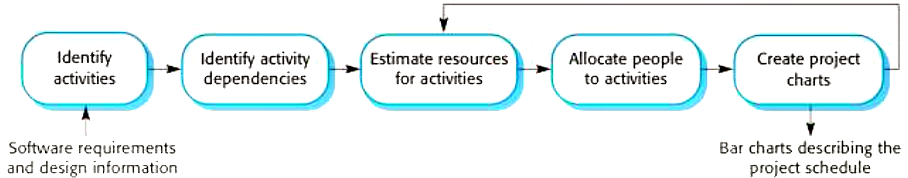
\includegraphics[width=0.75\textwidth]{mainmatter/pics/project_shedulding.png}
    \caption{Project schedulding}
\end{figure}

\subsubsection{Milestones und Deliverables:}
\begin{itemize}
    \item \textbf{Milestones:} Punkte im Zeitplan, dienen zur Bewertung des Fortschrittes
    \item \textbf{Deliverables:} Erzeugnisse, die an den Kunden ausgeliefert werden (Requirements documents)
\end{itemize}

\subsubsection{Probleme:}
\begin{itemize}
    \item Abschätzung des Ausmaßes von Problemen und damit der Kosten für ihre Lösung ist schwierig
    \item Produktivität ist nicht proportional zur Auswahl der Mitarbeiter 
    \item Einsatz von zusätzlichen Arbeitskräften bei einem verspäteten Projekt führt zu zusätzlicher Verspätung (Kommunkations-Overhead)
    \item Murphy's Law: möglichst alle Eventualitäten einplanen
\end{itemize}

\subsection{Agile Planung: Schritte}
\begin{itemize}
    \item \textbf{Agile Planung:} inkrementelle Planung, Prozess kann bei veränderten Anforderungen abgeändert werden
    \item \textbf{Planung der Veröffentlichung:} mehrere Monate im Voraus, bestimmt die in der Veröffentlichung inbegriffenen Funktionen
    \item \textbf{Planung der Iterationen:} kurzfristig, Planung es nächsten Inkrements (2-4 Wochen Arbeitszeit)
    \item \textbf{Extreme Programming (XP):} Story-basierte Planung 
\end{itemize}

\subsection{Key Points:}
\begin{itemize}
    \item Preis für Software wird nicht nur durch Entwicklungskosten bestimmt, sondern kann durch Markt- oder Unternehmensprioritäten beeinflusst werden. 
    \item Planungsgesteuertes entwickeln wird um inen kompletten Projektplan organisiert, definiert Projektaktivitäten, Aufwand, Zeitplan und Aufgabenverteilung
    \item Erstellung des Zeitplans mit Hilfe von graphischen Darstellungen des Projektplans 
    \item XP-Planspiel beteiligt das gesamte Team an der Projektplanung. Plan wird inkrementell entwickelt, wird bei auftretenden Problemen angepasst (Reduzierung von Funktionalitäten anstatt Verzögerung der Auslieferung)
\end{itemize}

\section{Techniken zur Aufwandsabschätzung}
\textbf{\large{Zwei Arten:}}
\begin{itemize}
    \item \textit{Erfahrungsbasiert:} Abschätzung des benötigten Aufwandes abhängig von Erfahrung des Projektleiters und des Anwendungsbereiches der Software 
    \item \textit{Algorithmische Kostenmodellierung:} formelähnliche Herangehensweise zur berechnung des Arbeitsaufwandes, basierend auf Abschätzung von Projektattributen (Größe, Erfahrung der Mitarbeiter, \dots)
\end{itemize}

\subsection{Algorithmische Kostenmodellierung}
\begin{itemize}
    \item Mathematische Funktion aus Produkt, Projekt, Prozessatributen. Werte werden vom Projektleiter abgeschätzt
    \item $A \times Size^{B} \times M$
    \begin{itemize}
        \item $A$: organisationsabhägige Konstante
        \item $B$: spiegelt den uvnerhätlnismäßigen Aufwand für große Projekte wieder
        \item $M$: Multiplikator, spiegelt Produkt-, Pozess- und Personalattribute wieder 
    \end{itemize}
    \item \textcolor{red}{Häufigstes Produktattribut: Codegröße}
    \item Modelle meist ähnlich, aber unterschiedliche Werte für $A$, $B$ und $M$
\end{itemize}

\subsection{Genauigkeit der Abschätzung}
\begin{itemize}
    \item Größe einer Sfotware erst nach Fertigstellung bekannt
    \item beeinflussende Faktoren:
    \begin{itemize} 
        \item Verwendung von COTS und bereits existierenden Komponenten 
        \item Programmiersprache
        \item Verteilung des Systems
    \end{itemize}
    \item je weiter der Entwicklungsprozess fortgeschritten ist, desot genauer kann die codegröße abgeschätzt werden 
    \item Abschätzungen der zu $B$ und $M$ gehörenden Faktoren subjektiv
\end{itemize}

\subsubsection{COCOMO 2}
\begin{itemize}
    \item empirisches Modell, erfahrungsbasiert
    \item gut dokumentiert, unabhängig
    \item mehrfah überarbeitet
    \item berückstichtigt verschiedene Herangehensweisen an softwareentwicklung, Wiederverwendung etc.
    \item enthält eine Anzahl von Untermodellen $\rightarrow$ zunehmend detailliertere Abschätzungen 
    \item Untermodelle:
    \begin{enumerate}
        \item \textbf{Application-composition-Modell} \\
        zusammensetzen von Software aus bereits existierenden Teilen
        \item \textbf{Frühes Designmodell} \\
        Anforderungen verfügbar, aber Designprozess noch nicht begonnen
        \item \textbf{Reuse-Modell} \\
        Berechnung des Aufwandes, wiederverwendbare Komponenten zu integrieren
        \item \textbf{Post-architecture-Modell}\\
        nach Design der Systemarchitektur $\rightarrow$ mehr Infromation über das System verfügbar
    \end{enumerate}
\end{itemize}
\begin{figure}[h]
    \centering
    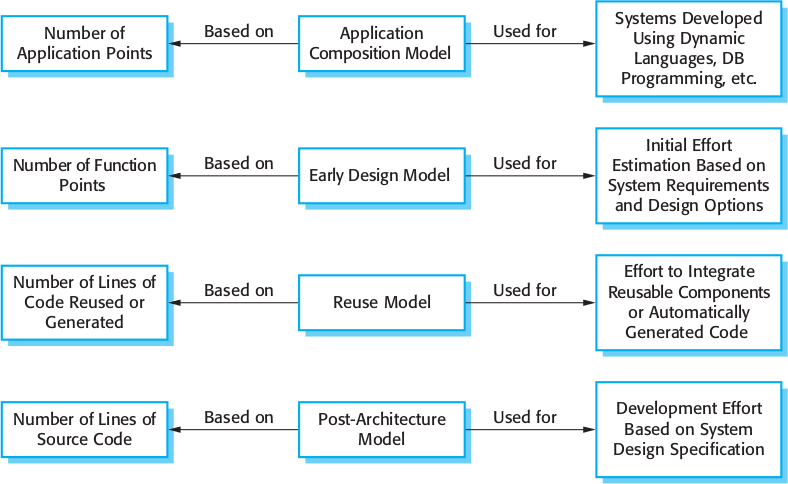
\includegraphics[width=0.75\textwidth]{mainmatter/pics/cocomo.png}
    \caption{COCOMO estimation models}
\end{figure}

\subsubsection{Application composition-Modell}
